\section{Oscillation inherent in DFT}
\label{DFToscillation} 
Let there be a voltage signal defined as
\begin{align}
v(t) &= V_m\cos(2\pi f t + \phi)\nonumber\\
\intertext{Therefore we write it as}
v(t) &= V_m \frac{e^{j(\omega t + \phi)}+e^{-j(\omega t + \phi)}}{2}\nonumber\\
\intertext{Now if we apply DFT on the signal taking the first sample of the $l^{th}$ window as the starting point. Let us define $k$ as}
k &= \frac{f}{f_o}\nonumber\\
\intertext{and N as the number of samples per cycle assuming system to be at nominal frequency. Now applying full cycle DFT on the signal,in discrete domain,we have}
\label{dft}
V_1^w &= V_m\frac{1}{N}\left[e^{j\phi}\sum_{n=w}^{N-w+l} e^{j\frac{2\pi(k-1)}{N}n}\right]\nonumber\\
&+ V_m\frac{1}{N}\left[e^{-j\phi}\sum_{n=w}^{N-w+l} e^{-j\frac{2\pi(k+1)}{N}n}\right]
\intertext{The above expression simplifies as follows (for detailed analysis refer \ref{simplifying}).}
\label{simplify}
V_1^w &= V_m\frac{1}{N}e^{j(\phi+\frac{2\pi(k-1)(w-\frac{N}{2})}{\frac{N}{2}})}
\left[\frac{\sin(\pi(k-1))}{\sin(\frac{\pi(k-1)}{N})}\right]\\
&+ V_m\frac{1}{N} e^{-j(\phi +\frac{2\pi(k+1)(w-\frac{N}{2})}{\frac{N}{2}})} \left[\frac{\sin(\pi(k+1))}{\sin(\frac{\pi(k+1)}{N})}\right]
\end{align}
Now we define
\begin{align*}
A&=\frac{1}{N}\frac{\sin(\pi(k-1))}{\sin(\frac{\pi(k-1)}{N})}\\
B&=\frac{1}{N}\frac{\sin(\pi(k+1))}{\sin(\frac{\pi(k+1)}{N})}\\
\psi_1^w&=\frac{2\pi(k-1)(w-\frac{N}{2})}{\frac{N}{2}}\\
\psi_2^w&= \frac{2\pi(k+1)(w-\frac{N}{2})}{\frac{N}{2}}\\
\end{align*}
Now the magnitude of the phasor is given as $ V^w.V^{w*}$ or
\begin{align*}
V^w_l.V_l^{w*}&=|V_1^w|^2=V_m^2[Ae^{j(\phi+\psi^w_1)} + Be^{-j(\phi+\psi^w_2)}]\\
& [Ae^{-j(\phi+\psi^w_1)} + Be^{+j(\phi+\psi^w_2)}]
\intertext{or}
V^w_l.V_l^{w*}&=|V_1^w|^2=V_m^2\left[(A^2+B^2)\right]\\
 &+ V_m^2\left[AB(e^{j(2\phi+\psi_1^w+\psi_2^w)} + e^{-j(2\phi+\psi_1^w +\psi_2^w)})\right]
\end{align*}
Now in this magnitude expression we have a constant part i.e.$(A^2+B^2)$ and a variable part which is dependant on the windownumber(i.e. $e^{j(2\phi+\psi_1^w+\psi_2^w)} + e^{-j(2\phi+\psi_1^w +\psi_2^w)}$ ). This part manifests as oscillation in the output. This anomaly is inherent in the DFT process. One way to eliminate these oscillations is to use three phase information.
\begin{equation}
|\tilde{V}|=\sqrt{\frac{|V_A^w|^2 + |V_B^w|^2 + |V_C^w|^2}{3}}
\end{equation}
It can be easily shown that
\begin{align*}
V_A^wV_A^{w*} &= |V_{A}^w|^2=V_m^2\left[(A^2+B^2)\right]\\
  &+ V_m^2\left[AB[e^{j2\phi}e^{j(\psi_1^w +\psi_2^w)}+ e^{-j 2\phi } e^{-j (\psi_1^w+\psi_2^w)}]   \right]\\
V_B^wV_B^{w*} &= |V_{B}^w|^2=V_m^2\left[(A^2+B^2)\right]\\
  &+ V_m^2\left[AB[e^{j2\phi}e^{j(\psi_1^w +\psi_2^w)} a + e^{-j 2\phi } e^{-j (\psi_1^w+\psi_2^w)}a^2]\right]\\
V_C^wV_C^{w*} &= |V_{C}^w|^2=V_m^2\left[(A^2+B^2)\right]\\
  &+ V_m^2\left[AB[e^{j2\phi}e^{j(\psi_1^w +\psi_2^w)} a^2 + e^{-j 2\phi } e^{-j (\psi_1^w+\psi_2^w)}  a]\right]
\end{align*}
where $a=e^{j\frac{2\pi}{3}}$. Now adding the above three equations we have
%\begin{eqnarray*}
%&&|\tilde{V}|^2=V_m^2\left[3(A^2+B^2)+ (1+a+a^2) AB[e^{j2\phi}e^{j(\psi_1^w +\psi_2^w)}]\right]\\
%&& +V_m^2\left[(1+a+a^2) AB[e^{-j 2\phi } e^{-j (\psi_1^w+\psi_2^w)}]\right]
%\end{eqnarray*}
\begin{align*}
|\tilde{V}|^2 = V_m^2\left[3(A^2+B^2)+ (1+a+a^2) AB[e^{j2\phi}e^{j(\psi_1^w +\psi_2^w)}]\right]\\
+ V_m^2\left[(1+a+a^2) AB[e^{-j 2\phi } e^{-j (\psi_1^w+\psi_2^w)}]\right]
\end{align*}
Therefore as ${\bf 1+a+a^2=0}$ the oscillatory components vanish and we get a stable output. Therefore we see that the factor that comes as ${\bf A^2+B^2}$ manifests as error in the measurement. Plotting ${\bf \sqrt{A^2+B^2}}$ for different values of frequency (i.e. between 47 Hz to 53 Hz) we see that the values of the expression comes almost close to 1 as shown in Fig. (\ref{accuracy}). Hence we can approximate $V_m$ as,
\begin{equation}
V_m^2=\frac{\tilde{V}^2}{3}
\end{equation}

The important point to note here is that the above analysis works only for balanced system. In case of an unbalanced system we should compute the balanced sequence components (positive sequence) using SCDFT (Sequence Components Discrete Fourier Transform).
\begin{figure}[!t]
\centering
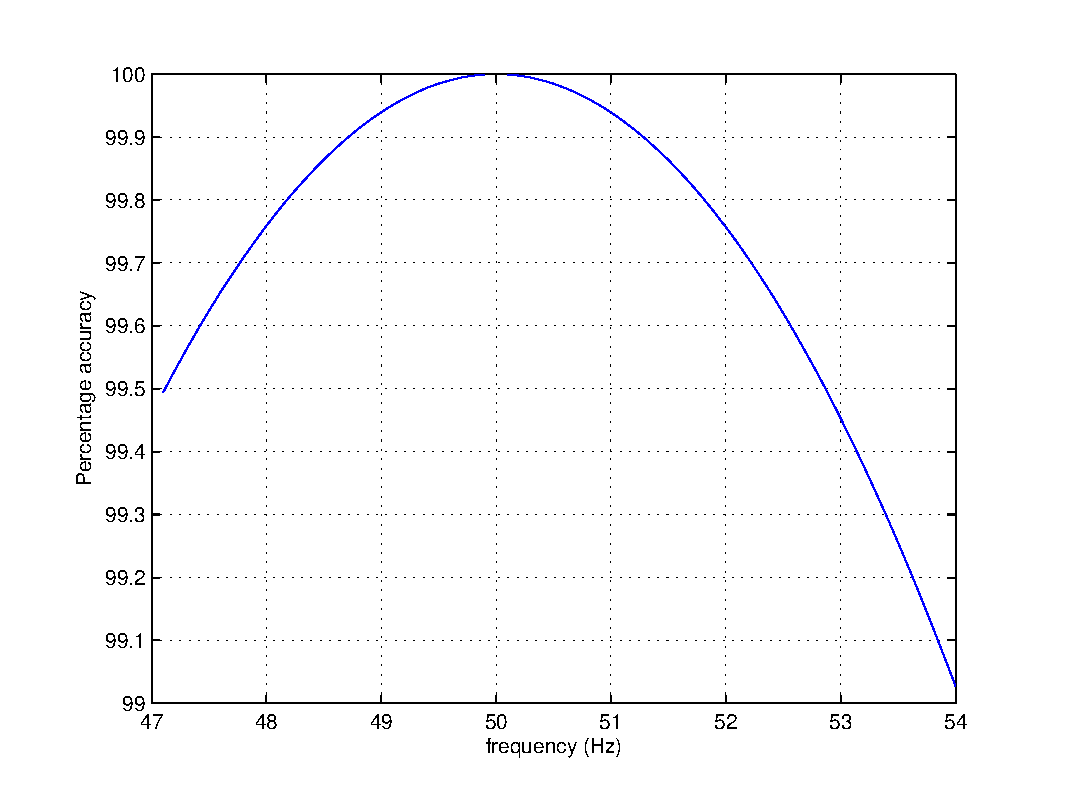
\includegraphics[width=3in]{percentage_accuracy}
\caption{Percentage Accuracy vs Frequency plot}
\label{accuracy}
\end{figure}


\section{Simplifying Equation}
\label{simplifying}
The expression obtained in (\ref{dft}) i.e.
\begin{align*}
V_1^w &= V_m\frac{1}{N}\left[e^{+j\phi}\sum_{n=w}^{N-w+l} e^{j\frac{2\pi(k-1)}{N}n}\right]\\
&+ V_m\frac{1}{N}\left[e^{-j\phi}\sum_{n=w}^{N-w+l} e^{-j\frac{2\pi(k+1)}{N}n}\right]
\end{align*}
can be solved as follows.
The first summation is infact a series summation of geometric progression which can be simplified as
\begin{align*}
S_1 &= \frac{2}{N}e^{+j\phi}\sum_{n=w}^{N-w+l} q^n\\
\intertext{where q is $e^{j 2\pi\frac{k-1}{N}n}$.Therefore we get $S_1$ as}
S_1 &= \frac{1}{N} e^{+j\phi} q^w\left[\frac{1-q^N}{1-q}\right]\\
\intertext{Similarly for the other summation $S_2$ we have}
S_2 &= \frac{1}{N} e^{-j\phi} p^w\left[\frac{1-p^N}{1-p}\right]
\end{align*}
where p is $e^{-j 2\pi\frac{k+1}{N}n}$. Therefore
\begin{align*}
V_1^w &= V_m\frac{1}{N} e^{+j\phi} q^w\left[\frac{1-q^N}{1-q}\right]\\
      &+ V_m\frac{1}{N} e^{-j\phi}p^w\left[\frac{1-p^N}{1-p}\right]\\
\intertext{Here $V_1^w$ is a function of w i.e. the window number. Again we can write}
V_1^w &= V_m\frac{1}{N} e^{+j\phi}q^w\frac{q^{\frac{N}{2}}}{q^\frac{1}{2}} \left[\frac{q^{-\frac{N}{2}}-q^{\frac{N}{2}}}{q^{-\frac{1}{2}}-q^{\frac{1}{2}}}\right]\\
&+ V_m\frac{1}{N} e^{-j\phi} p^w\frac{p^{\frac{N}{2}}}{p^{\frac{1}{2}}} \left[\frac{p^{-\frac{N}{2}}-p^{\frac{N}{2}}}{p^{-\frac{1}{2}}-p^{\frac{1}{2}}}\right]\\
\intertext{Now substituting the values of $p$ and $q$ we have the expression simplified as mentioned in (\ref{simplify}) i.e.}
V_1^w &= V_m\frac{1}{N} e^{+j(\phi +\frac{2\pi(k-1)(w-\frac{N}{2})}{\frac{N}{2}})} \left[\frac{\sin(\pi(k-1))}{\sin(\frac{\pi(k-1)}{N})}\right]\\
&+ V_m\frac{1}{N} e^{-j(\phi +\frac{2\pi(k+1)(w-\frac{N}{2})}{\frac{N}{2}})} \left[\frac{\sin(\pi(k+1))}{\sin(\frac{\pi(k+1)}{N})}\right]
\end{align*}

\section{Other algorithms on Frequency measurement}
Amongst the existing algorithms for frequency estimation the Phadke Thorp's method is the most popular. The basic idea behind Phadke Thorpe's method of frequency estimation is that if we take a DFT on the positive sequence voltage at offnominal frequencies then the obtained phasor rotates in the complex plane with an angular velocity which directly proportional to the frequency deviation. Let the nominal frequency be $\omega_o$.then we can write the phase voltages as,
\begin{align*}
V_a(t) &= \frac{1}{2}[Ve^{j\omega t}+V^*e^{-j\omega t}]\\
V_b(t) &= \frac{1}{2}[V\alpha ^2 e^{j\omega t}+V^*\alpha^{*2} e^{-j\omega t}]\\
V_c(t) &= \frac{1}{2}[V\alpha e^{j\omega t}+V^*\alpha^{*} e^{-j\omega t}]
\end{align*}where V is the positive sequence voltage and $\alpha$ is $e^{j\frac{2\pi}{3}}$,and $\omega$ is the offnominal frequency different from $\omega_o$. Now if we apply DFT to calculate the positive sequence voltage corresponding to N samples per cycle,for the $L^{th}$ window then we have
\begin{align*}
V^L = &\frac{2}{k}\sum_{n=l}^{N-1+l}\frac{1}{3}[V_a(N\Delta t)\\
&+\alpha V_b(N\Delta t)+\alpha^2 V_c(N\Delta t)]e^{-jn\omega_o\Delta t}\\
\intertext{Now substituting the values of $V_a$, $V_b$ and $V_c$ we get the following simplified form,}
V^L = &\frac{1}{N}\sum_{n=l}^{N-1+l}V e^{jn\Delta\omega\Delta t}
\end{align*}
This sum can be computed as
\begin{equation}
\label{bracket}
V^L=Ve^{jl\Delta\omega\Delta t}\left[\frac{\sin(\frac{N\Delta\omega\Delta t}{2})}{N\sin(\sin(\frac{N\Delta\omega\Delta t}{2})} e^{-j(N-1)\Delta\omega\frac{\Delta t}{2}}\right]
\end{equation}
The bracketed term in (\ref{bracket}) is the error in estimating the phasor. Therefore it is evident that the obtained phasor does have a rotation proportional to the frequency deviation.

Let the phase angle of the voltage phasor be $\psi$, then,
\begin{align*}
\psi_w&=\psi_{w-1} + \Delta\omega\Delta t
\intertext{or in other words}
\frac{d\psi}{dt}&=\frac{\psi_w - \psi_{w-1}}{\Delta t} = \Delta\omega
\end{align*}
Therefore we see that if $\Delta f$ is +1 then the phasor rotates counterclockwise in the plane at the rate of one revolution per second. If the $\Delta f$ is -1 then the rotation is clockwise. Now if the system is exposed to noise then merely differentiating the slope will further increase the error. Therefore as suggested it is advisable to wait for the phasor to sweep over a certain angle and then take the measurements. In their method they have suggested an angle of 0.5 radians, on which case the time required for measurement comes out to be
\begin{equation}
\label{qwert}
T=\frac{0.5}{2\pi \Delta f}
\end{equation}
Therefore it is evident that smaller frequency deviations will take larger time to measure and larger deviations smaller.

\section{Recursive update}
\label{rec_update}
Referring to Phadke Thorp's method a recursive update for SC DFT can be stated as,
\begin{align*}
&V_{Ac}^{w+1}(m) = V_{Ac}^{w}(m)\\
&+\frac{2}{18N}\left[(v_w^A-v_{w-N}^A)\cos((w-(N+1))\frac{2\pi m}{N})\right]\\
&+\frac{2}{18N}\left[(v_w^B-v_{w-N}^B)\cos((w-\frac{2N}{3}-(N+1))\frac{2\pi m}{N})\right]\\
&+\frac{2}{18N}\left[(v_w^C-v_{w-N}^C)\cos((w-\frac{N}{3}-(N+1))\frac{2\pi m}{N})\right]
\end{align*}
\begin{align*}
& V_{As}^{w+1}(m)=V_{As}^{w}(m)\\
&+\frac{2}{18N}\left[(v_w^A-v_{w-N}^A)\sin((w-(N+1))\frac{2\pi m}{N})\right]\\
&+\frac{2}{18N}\left[(v_w^B-v_{w-N}^B)\sin((w-\frac{2N}{3}-(N+1))\frac{2\pi m}{N})\right]\\
&+\frac{2}{18N}\left[(v_w^C-v_{w-N}^C)\sin((w-\frac{N}{3}-(N+1))\frac{2\pi m}{N})\right]
\end{align*}
Similarly for B phase,
\begin{align*}
& V_{Bc}^{w+1}(m)=V_{Bc}^{w}(m)\\
&+\frac{2}{18N}\left[(v_w^B-v_{w-N}^B)\cos((w-(N+1))\frac{2\pi m}{N})\right]\\
&+\frac{2}{18N}\left[(v_w^C-v_{w-N}^C)\cos((w-\frac{2N}{3}-(N+1))\frac{2\pi m}{N})\right]\\
&+\frac{2}{18N}\left[(v_w^A-v_{w-N}^A)\cos((w-\frac{N}{3}-(N+1))\frac{2\pi m}{N})\right]
\end{align*}
\begin{align*}
& V_{Bs}^{w+1}(m)=V_{Bs}^{w}(m)\\
&+\frac{2}{18N}\left[(v_w^B-v_{w-N}^B)\sin((w-(N+1))\frac{2\pi m}{N})\right]\\
&+\frac{2}{18N}\left[(v_w^C-v_{w-N}^C)\sin((w-\frac{2N}{3}-(N+1))\frac{2\pi m}{N})\right]\\
&+\frac{2}{18N}\left[(v_w^A-v_{w-N}^A)\sin((w-\frac{N}{3}-(N+1))\frac{2\pi m}{N})\right]
\end{align*}
and for C phase,
\begin{align*}
& V_{Cc}^{w+1}(m)=V_{Cc}^{w}(m)\\
&+\frac{2}{18N}\left[(v_w^C-v_{w-N}^C)\cos((w-(N+1))\frac{2\pi m}{N})\right]\\
&+\frac{2}{18N}\left[(v_w^A-v_{w-N}^A)\cos((w-\frac{2N}{3}-(N+1))\frac{2\pi m}{N})\right]\\
&+\frac{2}{18N}\left[(v_w^B-v_{w-N}^B)\cos((w-\frac{N}{3}-(N+1))\frac{2\pi m}{N})\right]
\end{align*}
\begin{align*}
& V_{Cs}^{w+1}(m)=V_{Cs}^{w}(m)\\
&+\frac{2}{18N}\left[(v_w^C-v_{w-N}^C)\sin((w-(N+1))\frac{2\pi m}{N})\right]\\
&+\frac{2}{18N}\left[(v_w^A-v_{w-N}^A)\sin((w-\frac{2N}{3}-(N+1))\frac{2\pi m}{N})\right]\\
&+\frac{2}{18N}\left[(v_w^B-v_{w-N}^B)\sin((w-\frac{N}{3}-(N+1))\frac{2\pi m}{N})\right]
\end{align*}


